% !TEX program = xelatex
\documentclass{article}

% Used packages
\usepackage{geometry}
\usepackage{fancyhdr}
\usepackage{lastpage}
\usepackage[scaled]{helvet}
\usepackage[T1]{fontenc}
\usepackage{hyperref}
\usepackage{indentfirst}
\usepackage{graphicx}
\usepackage{subcaption}

% Document info
\newcommand{\doctitle}{Convolutional Neural Network for Dog Breed Classification}
\newcommand{\docsubtitle}{Udacity Machine Learning Engineer Nanodegree Capstone Project}
\newcommand{\docauthor}{Alex Augusto Costa Machado}
\newcommand{\docdate}{December 10\textsuperscript{th} 2021}

% Page and margin setup
\geometry{
    a4paper,
    left=2cm,
    right=2cm,
    top=2cm,
    bottom=2cm,
    headsep=3mm,
    headheight=1.15cm
    }

% Paragraph setup
\setlength{\parindent}{2.5em}
\renewcommand{\baselinestretch}{1.25}

% Hyperlink setup
\hypersetup{
    colorlinks=true,
    linkcolor=black,
    urlcolor=blue,
    }
    
% Font setup
\renewcommand\familydefault{\sfdefault} 

% Header and footer setup
\pagestyle{fancy}
\fancyhf{}
\rhead{{\doctitle}}
\rfoot{\thepage\ / \pageref*{LastPage}}
\renewcommand{\footrulewidth}{0.4pt}

% First page setup
\newcommand{\docinfo}{
    \thispagestyle{empty}

    \begin{center}

        \Huge\textbf{\doctitle}
        \vspace{2mm}

        \LARGE\textbf{\docsubtitle}
        
        \vspace{3mm}
        \large
        Written by \textbf{\docauthor} on \textbf{\docdate}

    \end{center}
}

% Document
\begin{document}
    \docinfo

    \section{Definition}
    \subsection{Project Overview}

    For computer vision tasks, such as a dog breed classification, an algorithm mostly used is a Convolutional Neural Network, or CNN for short, which is a model that extracts features, like texture and edges, from spatial data.

    The history behind this algorithm started during the 1950s, but it is around the year 2012 that CNNs saw a huge surge in popularity after a CNN called AlexNet achieved state-of-the-art performance labeling pictures in the \href{https://image-net.org/}{ImageNet} challenge. Alex Krizhevsky et al. published the paper "ImageNet Classification with Deep Convolutional Neural Networks" describing the winning AlexNet model.

    \subsection{Problem Statement}

    The purpose of this project is to use a Convolutional Neural Network to classify dog breeds using images as input. For images that contain a human instead of a dog, the algorithm should display which dog breed resembles the human in the picture.

    \subsection{Metrics}

    The metric to evaluate the quality of the classifier is the accuracy of the dog breed predictions. The accuracy can be used in this case because the training data is not imbalanced. The definition of prediction accuracy is as follows:

    \[Accuracy = \frac{TP + TN}{TP +  TN + FP + FN} \]

    Where TP = True Positives, TN = True Negatives, FP = False Positives, and FN = False Negatives.

    \section{Analysis}

    \subsection{Data Exploration}

    There are two datasets for this project: one is a dog dataset containing 8351 images of 133 different dog breeds, and the other is a human dataset consisting of 13233 photos of 5749 different people. The dog dataset is divided in train, validation, and test datasets.

    A sample of the dog dataset is presented in the Figure \ref{fig:dog_sample}.

    \begin{figure}[htbp]
        \centering
        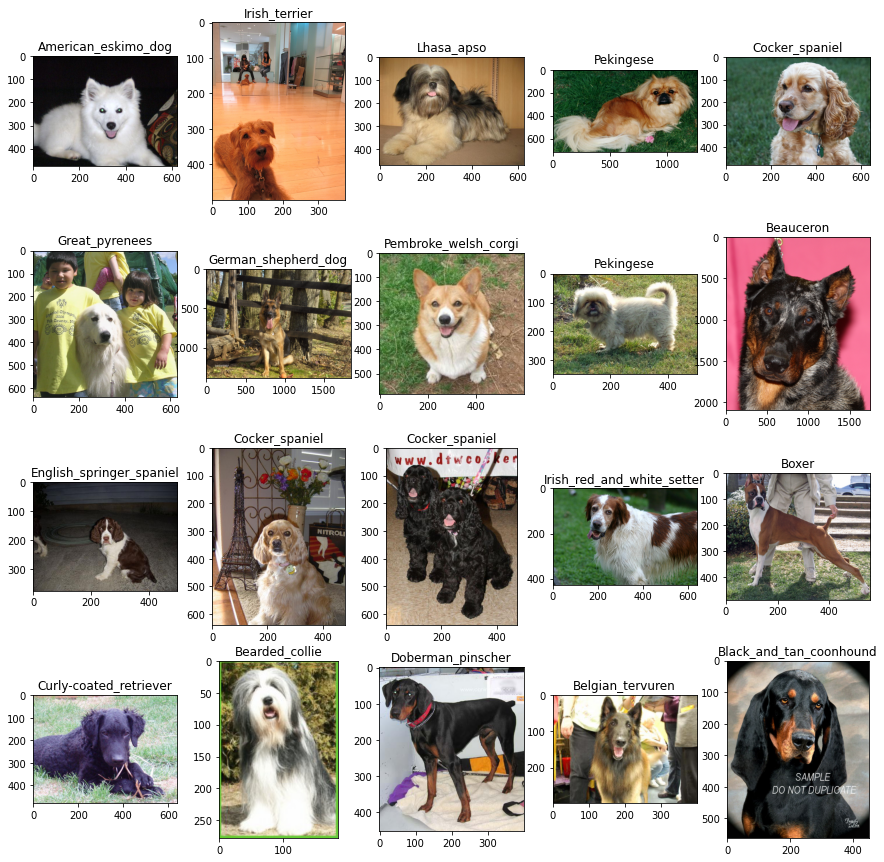
\includegraphics[width=\linewidth]{img/sample.png}
        \caption{Dog dataset sample.}
        \label{fig:dog_sample}
    \end{figure}

    \subsection{Exploratory Visualization}

    A way to explore this image dataset is to verify how many images there are for each of the dog breeds. The Figure \ref{fig:image_count} presents a graph of image count for each dog breed.

    \begin{figure}[htbp]
        \centering
        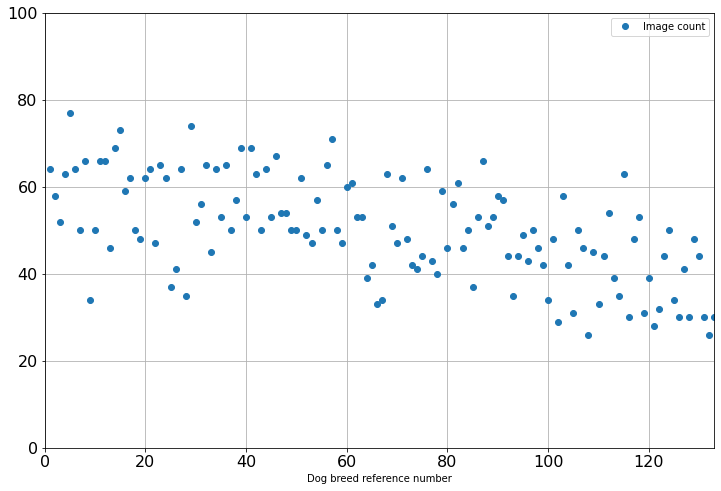
\includegraphics[width=\linewidth]{img/image_count.png}
        \caption{Number of images for each dog breed.}
        \label{fig:image_count}
    \end{figure}
    
    The Table \ref{tab:statistics} shows some statistical analysis of the number of images for each dog breed.

    \begin{table}[htbp]
        \centering
        \begin{tabular}{c|c}
             & \textbf{Value} \\
            \hline
            \textbf{Minimum} & 26 \\
            \textbf{Maximum} & 77 \\
            \textbf{Mean} & 50.23 \\
            \textbf{Median} & 50 \\
        \end{tabular}
        \caption{Statistical analysis of data.}
        \label{tab:statistics}
    \end{table}

    \subsection{Algorithms and Techniques}
    
    Three main algorithms will be used for this project: a human face detector, a dog detector, and a dog breed classifier.
    
    For the human face detector, I used an OpenCV's implementation of Haar feature-based cascade classifier. The pre-trained face detector is stored as XML file on \href{https://github.com/opencv/opencv/tree/master/data/haarcascades}{GitHub}.

    The dog detector and the dog breed classifier use VGG (Visual Geometry Group) pre-trained models with weights that have been trained on \href{https://image-net.org/}{ImageNet}, a very popular dataset used for image classification and other vision tasks.

    More about these two techniques is presented on the following sections.
    
    \subsubsection{Haar Feature-Based Cascade Classifiers}

    Haar feature-based cascade classifiers is an effective method for object detection proposed by Paul Viola and Michael Jones in their paper, "Rapid Object Detection using a Boosted Cascade of Simple Features" in 2001. It is a machine learning based approach where a cascade function is trained from a lot of positive and negative images. It is then used to detect objects in other images.

    Initially, the algorithm needs a lot of positive images (images of faces) and negative images (images without faces) to train the classifier. Then, the features are extracted from it using Haar features presented on Figure \ref{fig:haar_features}. Each feature is a single value obtained by subtracting sum of pixels under the white rectangle from sum of pixels under the black rectangle.

    \begin{figure}[htbp]
        \centering
        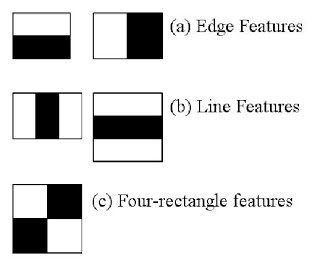
\includegraphics[width=.4\linewidth]{img/haar_features.jpg}
        \caption{Haar features.}
        \label{fig:haar_features}
    \end{figure}

    For each feature, it finds the best threshold which will classify the faces to positive and negative. As there are errors or misclassifications, the features with minimum error rate are selected, which means they are the features that most accurately classify the face and non-face images. The final classifier is a weighted sum of these weak classifiers. It is called weak because it alone can't classify the image, but together with others forms a strong classifier. The paper mentioned above states that even 200 features provide detection with 95\% accuracy.

    \subsubsection{Visual Geometry Group}

    Before talking about VGG, it is important to comment about AlexNet, which is a CNN used for image recognition that came out in 2012. It takes into account overfitting by using data augmentation and dropout. It replaces tanh activation function with ReLU by encapsulating its distinct features for over-pooling.
    
    VGG came into picture as it addresses the depth of CNNs. It is a pre-trained model and contains the weights that represent the features of whichever dataset it was trained on. More about the VGG architecture is presented below:

    \begin{itemize}
        \item Input: VGG takes in a 224x224 pixel RGB image. For the ImageNet competition, the authors cropped out the center 224x224 patch in each image to keep the input image size consistent.
        \item Convolutional Layers: the convolutional layers in VGG use a very small receptive field (3x3, the smallest possible size that still captures left/right and up/down). There are also 1x1 convolution filters which act as a linear transformation of the input, which is followed by a ReLU unit. The convolution stride is fixed to 1 pixel so that the spatial resolution is preserved after convolution.
        \item Fully-Connected Layers: VGG has three fully-connected layers: the first two have 4096 channels each and the third has 1000 channels, 1 for each class.
        \item Hidden Layers: all of VGG's hidden layers use ReLU. VGG does not generally use Local Response Normalization (LRN), as LRN increases memory consumption and training time with no particular increase in accuracy.
    \end{itemize}

    VGG, while based off of AlexNet, has several differences that separates it from other competing models:

    \begin{itemize}
        \item Instead of using large receptive fields like AlexNet (11x11 with a stride of 4), VGG uses very small receptive fields (3x3 with a stride of 1). Because there are now three ReLU units instead of just one, the decision function is more discriminative.
        \item VGG incorporates 1x1 convolutional layers to make the decision function more non-linear without changing the receptive fields.
        \item The small-size convolution filters allows VGG to have a large number of weight layers.
    \end{itemize}
    
    \subsection{Benchmark}
    
    The benchmark for the dog breed classifier will be a simple CNN model designed from scratch that will be compared to the final CNN obtained from transfer learning using a pre-trained VGG-11 model.
    
    The baseline model contains three convolutional blocks, each presenting a convolutional layer, a batch normalization layer, and a pooling layer. After these blocks, there is a dropout layer and a fully connected linear layer. A summary of the model is presented on Figure \ref{fig:model_summary}.
    
    \begin{figure}[htbp]
        \centering
        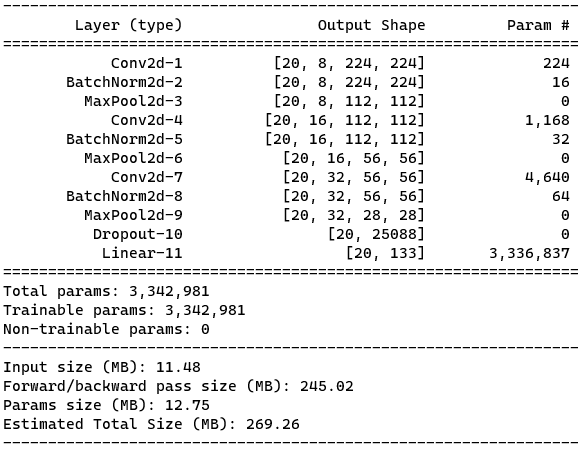
\includegraphics{img/model_summary.png}
        \caption{Summary of the benchmark model.}
        \label{fig:model_summary}
    \end{figure}
    
    \section{Methodology}

    \subsection{Data Preprocessing}

    Since the images have all different sizes, it was necessary to resize them. The images on the validation and testing datasets were resized to 256 pixels and cropped to square shapes of 224x224 pixels about the center and transformed into tensors, then the resulting tensors were normalized. A code snippet is presented on Figure \ref{fig:transform_train_test}.

    \begin{figure}[htbp]
        \centering
        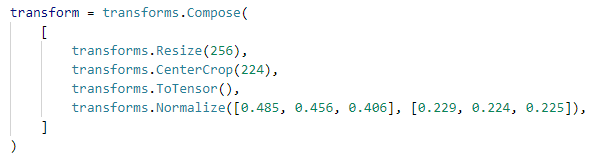
\includegraphics{img/transform_valid_test.png}
        \caption{Code for validation and testing transform.}
        \label{fig:transform_train_test}
    \end{figure}
    
    For the training data, in addition the resizing, cropping and normalization, data augmentation was applied, so the images were also randomly rotated and horizontally flipped. The Figure \ref{fig:transform_train} presents the code used for this transformation.
    
    \begin{figure}[htbp]
        \centering
        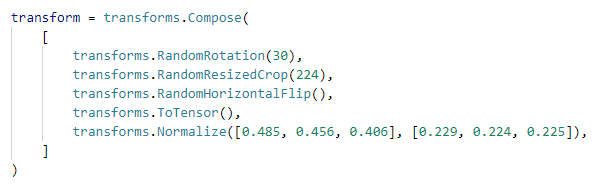
\includegraphics{img/transform_train.png}
        \caption{Code for training transform.}
        \label{fig:transform_train}
    \end{figure}

    \subsection{Implementation}

    \subsubsection{Human Face Detector}

    For the implementation of this algorithm I used an OpenCV's implementation of Haar feature-based cascade classifiers to detect human faces in images.

    The cascade classifier was downloaded from OpenCV's GitHub page and attached to a model. Then, the images were read and converted to grayscale. These images were then passed through to the model so that it could look up for faces in the pictures.

    After this, a bounding box was drawn around each face and the images were converted back to RGB so they could be plotted.

    No hyperparameters were changed for this, since there was no training needed for this model.
    
    \subsubsection{Dog Detector}
    
    A pre-trained VGG-16 model was used for this implementation. This model was downloaded along with weights that have been trained on ImageNet, a very large, very popular dataset used for image classification and other vision tasks. ImageNet contains over 10 million URLs, each linking to an image containing an object from one of 1000 categories.
    
    No hyperparameters were changed for this, since there was no training needed for this model. Before sending the images to the model, a set of transformations were necessary:

    \begin{itemize}
        \item Resize to 256 pixel.
        \item Crop to a square of 224x224 pixels.
        \item Convert to tensor.
        \item Normalize tensors.
    \end{itemize}

    After this, the model would return one of the 1000 indices of classification. Looking at the \href{https://gist.github.com/yrevar/942d3a0ac09ec9e5eb3a}{dictionary}, one can notice that the categories corresponding to dogs appear in an uninterrupted sequence and correspond to dictionary keys 151-268, inclusive, to include all categories from "Chihuahua" to "Mexican hairless".  Thus, in order to check to see if an image is predicted to contain a dog by the pre-trained VGG-16 model, I needed only to check if the pre-trained model predicts an index between 151 and 268 (inclusive).

    \subsubsection{Dog Breed Classifier CNN from scratch}

    This dog breed classifier is a simple CNN model designed from scratch that will be compared to the final CNN obtained from transfer learning using a pre-trained VGG-11 model.

    At first, I started with one convolutional block consisting of a convolutional layer, a batch normalization layer and a pooling layer. The output of this block would pass through a dropout layer and finally a fully connected layer. I then realized that adding more convolutional blocks increasing the output channels would improve the performance, so I ended up with three of these convolutional blocks. The code for this model is presented on Figure \ref{fig:model_scratch}.

    \begin{figure}[htbp]
        \centering
        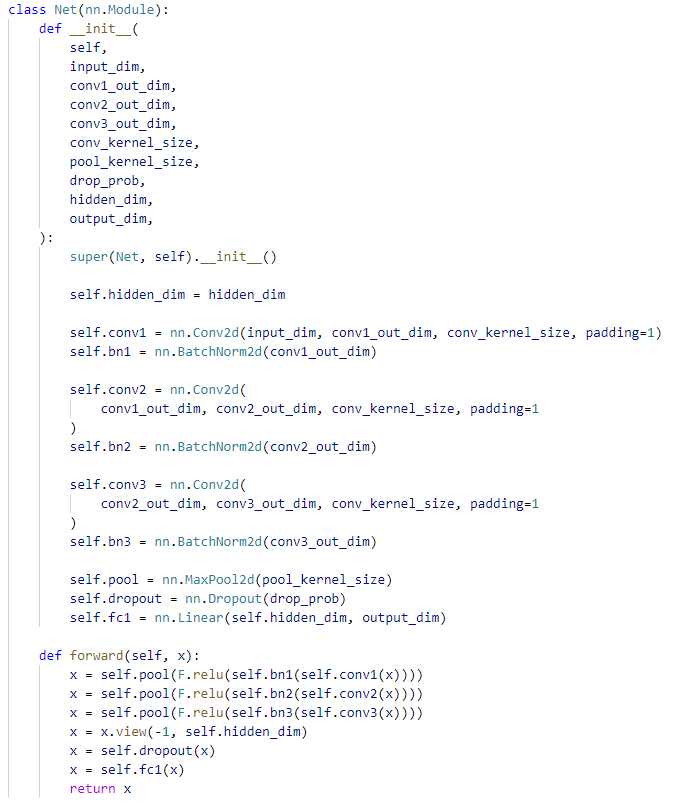
\includegraphics[width=\linewidth]{img/model_scratch.png}
        \caption{Code for CNN model made from scratch.}
        \label{fig:model_scratch}
    \end{figure}

    The hyperparameters used for this model are listed on Table \ref{tab:scratch_hyperparameters}.

    \begin{table}[htbp]
        \centering
        \begin{tabular}{c|c}
             \textbf{Hyperparameter} & \textbf{Value} \\
            \hline
            \textbf{input-dim} & 3 \\
            \textbf{conv1-out-dim} & 8 \\
            \textbf{conv2-out-dim} & 16 \\
            \textbf{conv3-out-dim} & 32 \\
            \textbf{conv-kernel-size} & 3 \\
            \textbf{pool-kernel-size} & 2 \\
            \textbf{drop-prob} & 0.5 \\
            \textbf{hidden-dim} & 25088 \\
            \textbf{output-dim} & 133 \\
        \end{tabular}
        \caption{Hyperparameters for CNN model from scratch.}
        \label{tab:scratch_hyperparameters}
    \end{table}

    For the loss function I used the cross entropy loss, and for optimization I used SGD with lr = 0.001 and momentum = 0.9.

    Each epoch of the training algorithm consists of a training step and a validation step, if the model presents a reduction on the validation loss, then the new parameters are saved.

    This model was trained for 80 epochs, reaching a validation loss of 3.561250 and an accuracy of 20\% when exposed to the test dataset.

    \subsubsection{Dog Breed Classifier CNN with Transfer Learning}

    A pre-trained VGG-11 model was used for this implementation. This model was downloaded along with weights that have been trained on ImageNet.

    After loading the model, it was necessary to freeze the existing parameters as to avoid destroying any of the information they contain during future training rounds.
    
    The final layer was overwritten, changing the output dimension to 133, which is the number of dog breeds in the training dataset. A summary for this model is presented on Figure \ref{fig:summary_transfer}.

    \begin{figure}[htbp]
        \centering
        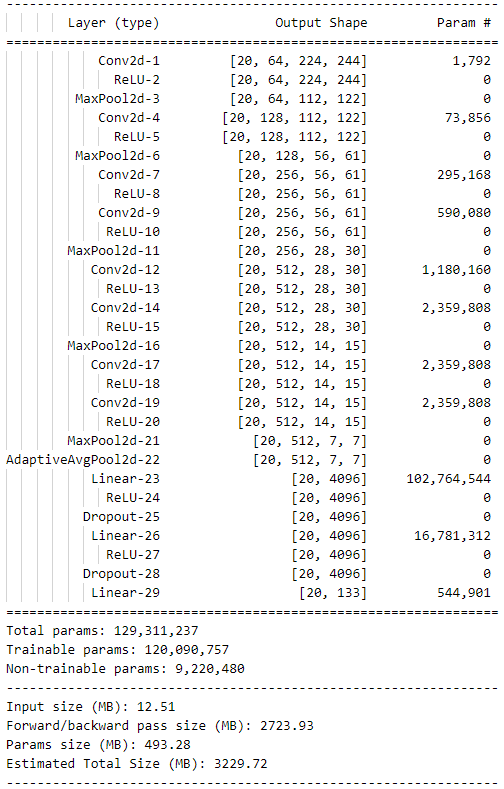
\includegraphics[height=650pt]{img/model_summary_transfer.png}
        \caption{Summary of the final model.}
        \label{fig:summary_transfer}
    \end{figure}

    For the loss function I used the cross entropy loss, and for optimization I used SGD with lr = 0.001 and momentum = 0.9.

    The training algorithm is the same as in the previous section: each epoch of consists of a training step and a validation step, every time the model presents a reduction on the validation loss, the new parameters are saved.

    This model was trained for 20 epochs, reaching a validation loss of 0.534802 and an accuracy of 86\% when exposed to the test dataset.

    \subsection{Refinement}

    When using transfer learning with the VGG-11 pre-trained model, at first it only reached 46\% of accuracy. Even trying to change the hyperparameters and batch size would make no difference on the final accuracy. What really made it reach 86\% was shuffling the training data before feeding it to the model.

    \section{Results}

    \subsection{Model Evaluation and Validation}

    The model achieved a prediction accuracy of 86\% when exposed to the test dataset. Using images of dogs chosen randomly on the Internet, I obtained the results presented on Table \ref{tab:target_pred}. Only two cases did not obtain the expected result (pictures 5 and 6), but the predicted dog breed is very similar to the target breed.
    
    On Figure \ref{fig:comparison_wrong} we can see the images for both cases. A Shih tzu (Figure \ref{fig:shih_tzu}) was provided as input, but a Lhasa apso (Figure \ref{fig:lhasa}) was predicted. The same happened for the Staffordshire bull terrier (Figure \ref{fig:staffy}) used as input and the American staffordshire terrier (Figure \ref{fig:american_staffy}) received as prediction.
    
    \begin{table}[htbp]
        \centering
        \begin{tabular}{c|c|c}
             & \textbf{Target} & \textbf{Prediction} \\
            \hline
            \textbf{Picture 1} & Alaskan malamute & Alaskan malamute \\
            \textbf{Picture 2} & French bulldog & French bulldog \\
            \textbf{Picture 3} & Afghan hound & Afghan hound \\
            \textbf{Picture 4} & Boxer & Boxer \\
            \textbf{Picture 5} & Shih tzu & Lhasa apso \\
            \textbf{Picture 6} & Staffordshire bull terrier & American staffordshire terrier \\
        \end{tabular}
        \caption{Comparison between target values and prediction results.}
        \label{tab:target_pred}
    \end{table}

    \begin{figure}[htbp]
        \centering
        \begin{subfigure}{.35\textwidth}
            \centering
            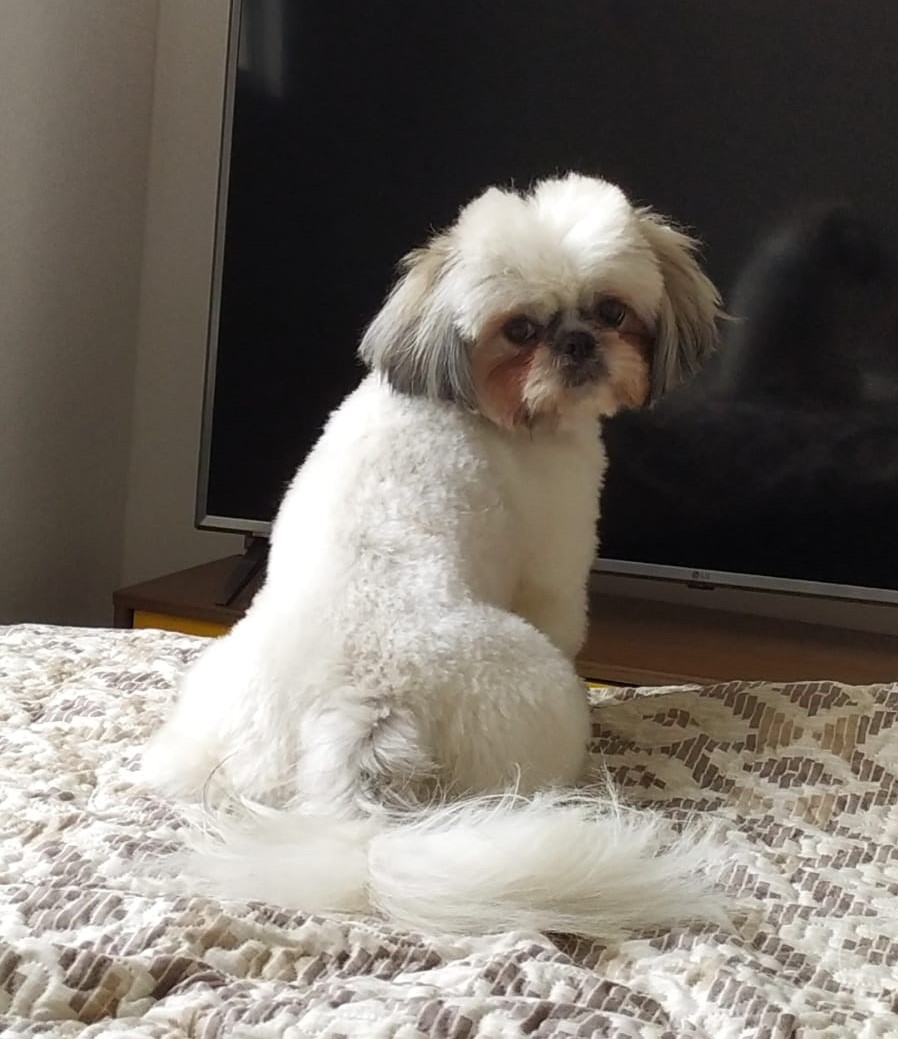
\includegraphics[width=\linewidth]{img/dog_shihtzu.jpeg}
            \caption{Target: Shih tzu}
            \label{fig:shih_tzu}
        \end{subfigure}%
        \hspace{0.1\textwidth}
        \begin{subfigure}{.45\textwidth}
            \centering
            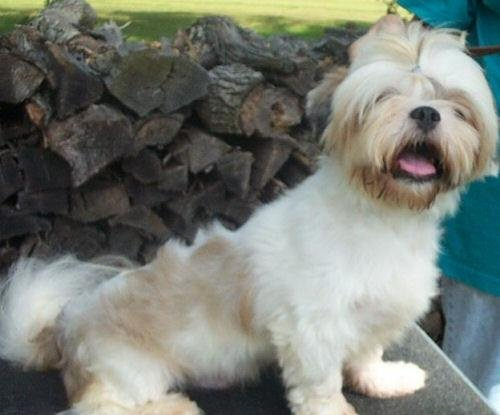
\includegraphics[width=\linewidth]{img/Lhasa_apso_06652.jpg}
            \caption{Prediction: Lhasa apso}
            \label{fig:lhasa}
        \end{subfigure}
        \begin{subfigure}{.35\textwidth}
            \centering
            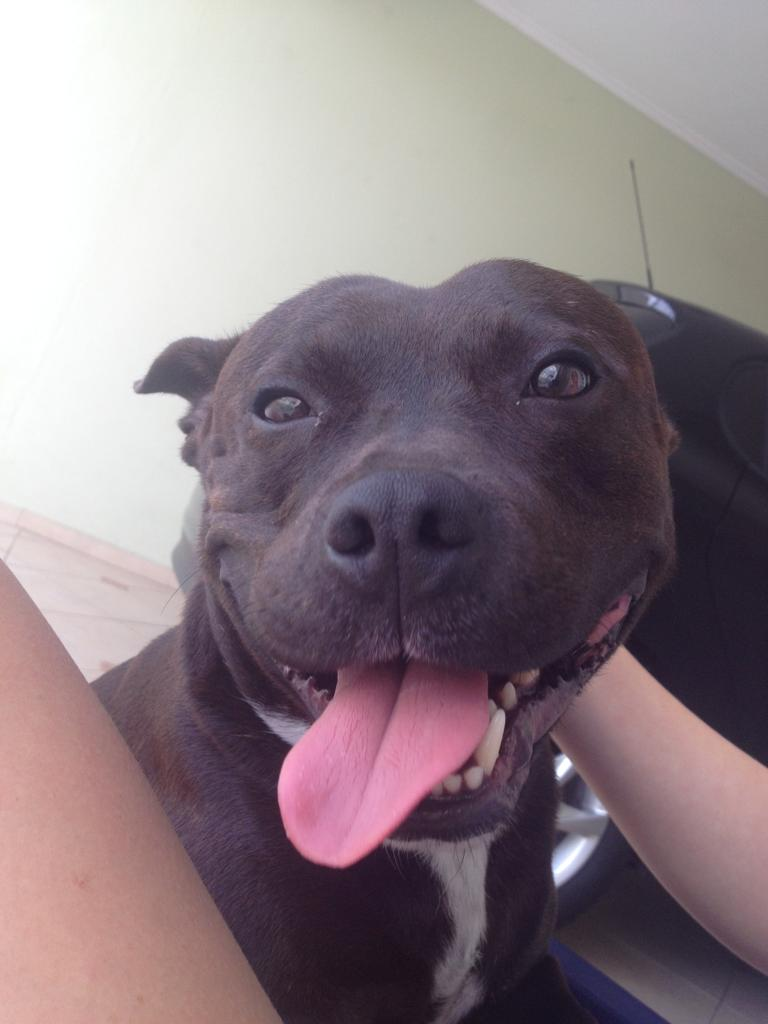
\includegraphics[width=\linewidth]{img/dog_staffordshire_bull_terrier.jpeg}
            \caption{Target: Staffordshire bull terrier}
            \label{fig:staffy}
        \end{subfigure}%
        \hspace{0.1\textwidth}
        \begin{subfigure}{.45\textwidth}
            \centering
            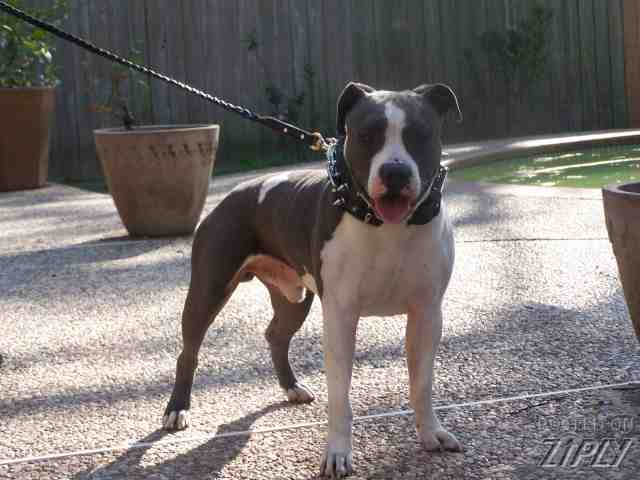
\includegraphics[width=\linewidth]{img/American_staffordshire_terrier_00548.jpg}
            \caption{Prediction: American staffordshire terrier}
            \label{fig:american_staffy}
        \end{subfigure}
        \caption{Comparison for wrongly classified dog breeds.}
        \label{fig:comparison_wrong}
    \end{figure}

    \subsection{Justification}

    The Table \ref{tab:results_comparison} presents a comparison between the results obtained for the proposed model and the benchmark model.

    \begin{table}[htbp]
        \centering
        \begin{tabular}{c|c|c}
             & \textbf{Benchmark model} & \textbf{Proposed model} \\
            \hline
            \textbf{Epochs} & 80 & 20 \\
            \textbf{Training loss} & 3.437396 & 0.830221 \\
            \textbf{Validation loss} & 3.561250 & 0.534802 \\
            \textbf{Test accuracy} & 20\% & 86\% \\
        \end{tabular}
        \caption{Comparison between benchmark and proposed models.}
        \label{tab:results_comparison}
    \end{table}

    It is possible to see that the proposed model performs a lot better than the benchmark model. As we used transfer learning, the model only required 20 epochs to reach an accuracy of 86\%, which is a satisfactory result.

    \section{Conclusion}

    \subsection{Reflection}

    This project was very important for me to understand the different steps of creating a machine learning model. From data exploration, to preprocessing, training, and testing, all the steps were included in this project.

    The most difficulty I had was making the configuration of the Convolutional Neural Network for the Python program to run correctly without any exceptions being raised.

    \subsection{Improvement}

    Some possible points of improvement are:

    \begin{itemize}
        \item Add functionality to detect dog mutts;
        \item Improve human face detection, as there were human faces detected on some dog images;
        \item Change the algorithm to try and reach over 90\% accuracy.
    \end{itemize}

\end{document}